%!TEX root=../document.tex

\subsection{Replikation}
(Geschrieben von Merna Zaher)

Ziel ist die Verteilung des LDAP-Schema auf mehr als einem Server. Dies erhöht die Ausfallsicherheit und verteilt die Last.
 

[VMware] Über rechtsklick auf der\verb| Vm-> Manage-> Cone| wird die Master-Vm dupliziert.


\begin{center}
	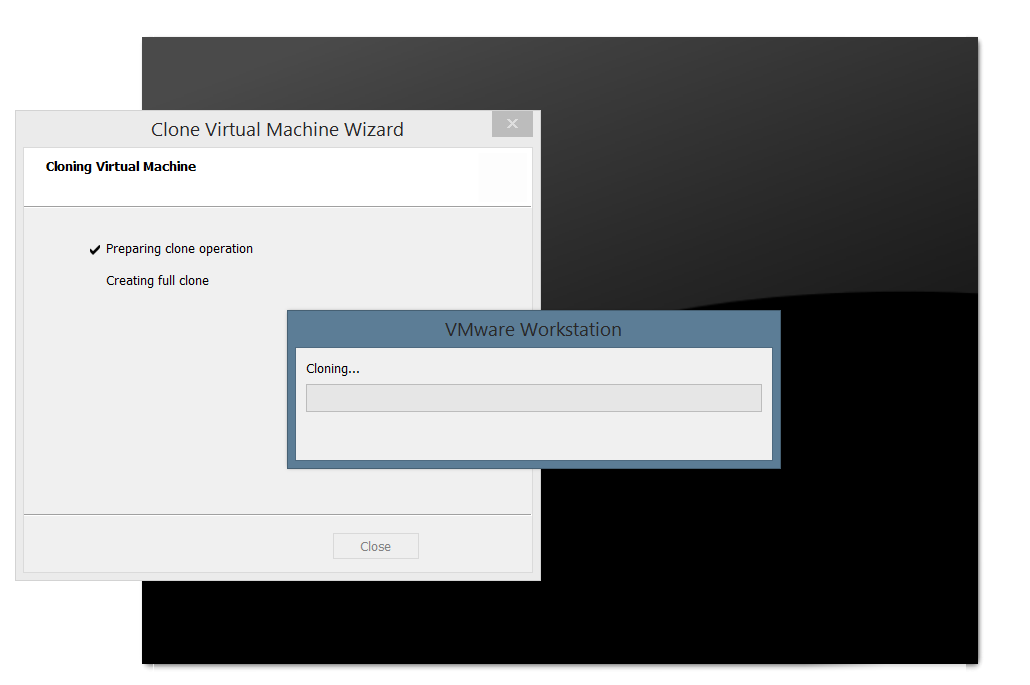
\includegraphics[width=0.75\linewidth]{images/a4_clonevirtualmachine.PNG}
\end{center}

Zunächst wird der eigene Domain-Name bzw ein eigener hostname eingerichtet sowie beim Master(der vorigen vm).Die selbe Struktur des Domainnamen wird eingehalten => sunaric.4chit.at\\
Damit der Name über DNS aufgelöst werden kann wird der Name und die dazugehörige ip-adresse der master-VM \textit{waldock} eingetragen.

Der Hostname wird sowohl in der /etc/hosts als auch in /etc/hostname umgeändert so wie bei der  Master-VM.
\begin{center}
	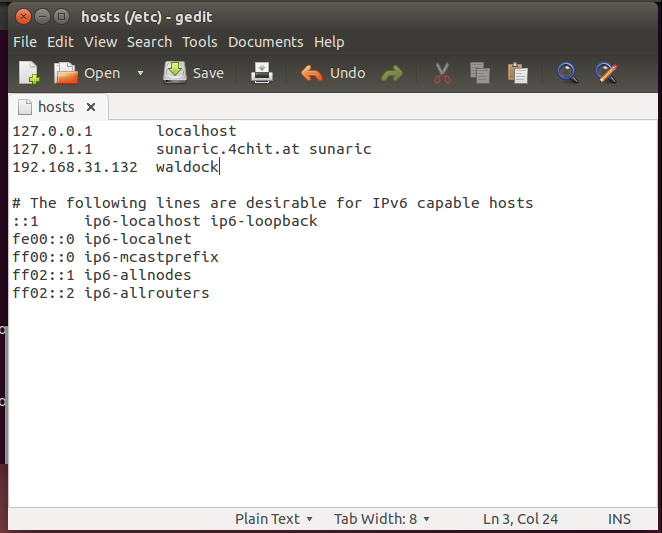
\includegraphics[width=1.0\linewidth]{images/a5_addmasterdns.PNG}
\end{center}


Hier wird überprüft ob der Hostname \textit{walddock} erstens aufgelöst werden kann und zweitens Zugriff auf die LDAP-Daten hat.


\begin{center}
	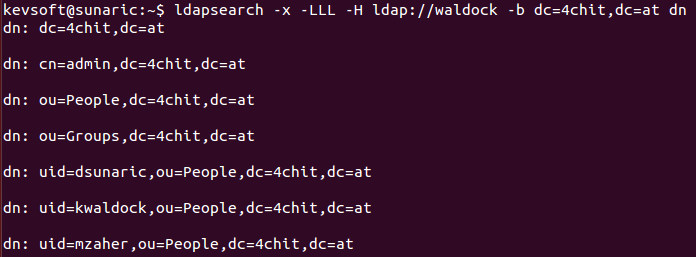
\includegraphics[width=1.0\linewidth]{images/a6_testaccessfromslavetomaster.PNG}
\end{center}

Wir haben uns entschieden die Replikation über eine ldif-Datei zu konfigurieren.\\Aufgrund dieser pro und contras:
\begin{itemize}
	\item[Pro   ] 
	\begin{itemize}
		\item Erlaubt Kommentare in der Konfiguration
		\item Einfach mit einem Texteditor Änderbar
		\item Im Besonderen sind Schema-Änderungen 
		leicht möglich
	\end{itemize}
	\item[Kontra]
		\begin{itemize}
			\item Statische Konfiguration → Erfordert Neustart 
			bei Änderungen
			\item Kann nicht auf andere Server repliziert werden
		\end{itemize}
\end{itemize}
Mittels \verb|ldapadd| wird eine ldif-Datei im system reingeladen die einen Acount für die Replikationsanfrage (\verb|cn=syncagent,dc=4chit,dc=at|)erstellt.

\begin{center}
	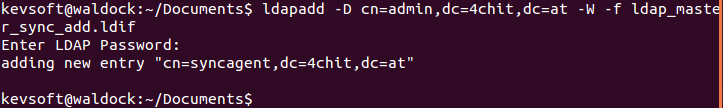
\includegraphics[width=1.0\linewidth]{images/a7_add_sync_account.PNG}
\end{center}

\begin{lstlisting}[escapechar=@]
@\bh@ Account fuer Replikationsabfrage@\eh@
dn: cn=syncagent,dc=4chit,dc=at
cn: syncagent
objectClass: top
objectClass: person
sn: syncagent
\end{lstlisting}
Hier wie man erkennen kann wird das auf der Server(Master)-vm \textit{kevsoft@waldock } geändert.
Über \verb|ldapmodify| kann die ldif-Datei modifiziert werden.
\begin{center}
	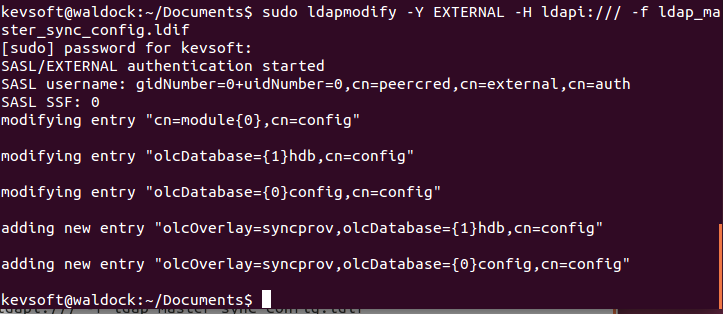
\includegraphics[width=1.0\linewidth]{images/a8_config_master_sync.PNG}
\end{center}

\begin{lstlisting}[escapechar=@]
      
@\bh@# Sync-Modul aktivieren@\eh@
dn: cn=module{0},cn=config
changetype: modify
add: olcModuleLoad
olcModuleLoad: syncprov.la
@\bh@.....@\eh@
@\bh@ #fuege replikationsrelevante Attribute zum Index hinzu @\eh@
dn: olcDatabase={1}hdb,cn=config
changetype: modify
add: olcDbIndex
olcDbIndex: entryUUID,entryCSN eq

@\bh@ # Zugriffsrechte fuer den sync-Account anlegen @\eh@
dn: olcDatabase={0}config,cn=config
changetype: modify
add: olcAccess
olcAccess: to * by dn.base="cn=syncagent,dc=4chit,dc=at" read by * +0 break

@\bh@# sync-Provider fuer die LDAP-Datenbank aktivieren@\eh@
dn: olcOverlay=syncprov,olcDatabase={1}hdb,cn=config
changetype: add
objectClass: olcOverlayConfig
objectClass: olcSyncProvConfig
olcOverlay: syncprov

@\bh@# sync-Provider fuer die LDAP-Konfiguration aktivieren@\eh@
dn: olcOverlay=syncprov,olcDatabase={0}config,cn=config
changetype: add
objectClass: olcOverlayConfig
objectClass: olcSyncProvConfig
olcOverlay: syncprov
\end{lstlisting}

Wie man erkennen kann wird das auf der Client-VM \textit{kevsoft@sunaric } geändert.
\begin{center}
	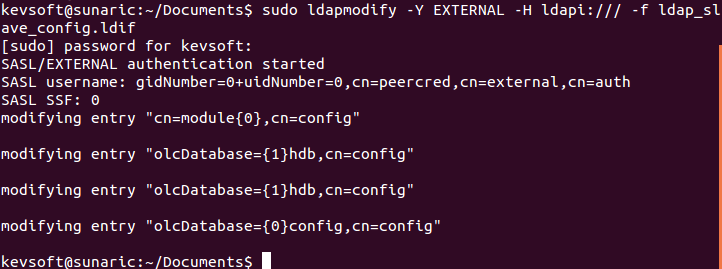
\includegraphics[width=1.0\linewidth]{images/a9_config_slave_sync.PNG}
\end{center}

\begin{lstlisting}[escapechar=@]

 @\bh@ #Sync-Modul aktivieren @\eh@
 dn: cn=module{0},cn=config
 changetype: modify
 add: olcModuleLoad
 olcModuleLoad: syncprov.la
 
@\bh@  # fuege replikationsrelevante Attribute zum Index hinzu@\eh@
 dn: olcDatabase={1}hdb,cn=config
 changetype: modify
 add: olcDbIndex
 olcDbIndex: entryUUID,entryCSN eq
 
@\bh@ # Datenbank-Replikation aktivieren@\eh@
 dn: olcDatabase={1}hdb,cn=config
 changetype: modify
 add: olcSyncrepl
 olcSyncrepl: {0}rid=2 provider=ldap://waldock
 type=refreshOnly
 bindmethod=simple
 binddn="cn=syncagent,dc=4chit,dc=at"
 credentials=123456
 interval="00:00:03:00"
 retry="30 10 300 +"
 timeout=1
 tls_reqcert=never
 schemachecking=off
 searchbase="dc=4chit,dc=at"
 
 @\bh@# Konfigurationsreplikation aktivieren@\eh@
 dn: olcDatabase={0}config,cn=config
 changetype: modify
 add: olcSyncrepl
 olcSyncrepl: {0}rid=1 provider=ldap://waldock
 type=refreshOnly
 bindmethod=simple
 binddn="cn=syncagent,dc=4chit,dc=at"
 credentials=123456
 interval="00:00:03:00"
 retry="30 10 300 +"
 timeout=1
 tls_reqcert=never
 schemachecking=off
 searchbase="cn=config"
\end{lstlisting}
 Über \verb|ldapsearch |kann man erkennen dass, der Client syncronisiert wurde .\\ \verb|dn: cn=syncagent,dc=4chit,dc=at|
\begin{center}
	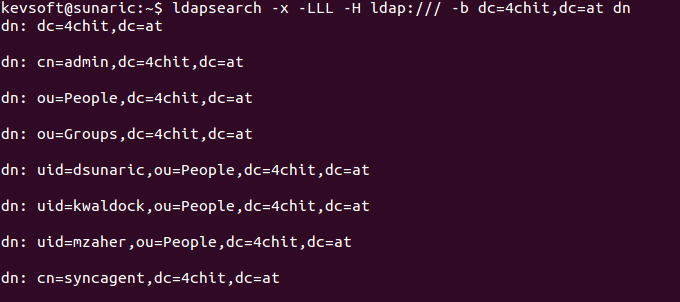
\includegraphics[width=1.0\linewidth]{images/a10_show_slave_sync_result_after_time.PNG}
\end{center}
